% IEEE standard conference template; to be used with:
%   spconf.sty  - LaTeX style file, and
%   IEEEbib.bst - IEEE bibliography style file.
% --------------------------------------------------------------------------

\documentclass[letterpaper]{article}
\usepackage{spconf,amsmath,amssymb,graphicx,xspace,tabularx,hyperref}
\usepackage{cleveref}
\let\cref=\Cref % Capitalise `Section 3` etc. when referencing
\crefname{figure}{fig.}{figs.}
\crefname{algocf}{algorithm}{algorithms}
\usepackage[sort&compress,numbers,sectionbib]{natbib}
\usepackage[ruled,noalgohanging,noend]{algorithm2e}
\usepackage{comment}
\input macros/todo
\input macros/macros
\overfullrule=2mm % black slugs on overfull lines, disable when submitting

% bold paragraph titles
\newcommand{\mypar}[1]{{\bf #1.}}
\newcommand{\myparcont}[1]{{\bf #1}}

% Title.
% ------
%\title{TODO: A Descriptive Title, not too general, not too long}
\title{Optimising Sequential Performance of\\ Belief Propagation for Top-N Recommendation}
%
% Single address.
% ---------------
\name{Henry Trinh, Richard Hladík, Stephanie Ruhstaller, Sarah Tr\"ondle}
\address{Department of Computer Science\\ ETH Zurich, Switzerland}

% For example:
% ------------
%\address{School\\
%		 Department\\
%		 Address}
%
% Two addresses (uncomment and modify for two-address case).
% ----------------------------------------------------------
%\twoauthors
%  {A. Author-one, B. Author-two\sthanks{Thanks to XYZ agency for funding.}}
%		 {School A-B\\
%		 Department A-B\\
%		 Address A-B}
%  {C. Author-three, D. Author-four\sthanks{The fourth author performed the work
%		 while at ...}}
%		 {School C-D\\
%		 Department C-D\\
%		 Address C-D}
%

\begin{document}
%\ninept
%
\maketitle
%


\begin{abstract}
	\begin{comment}Describe in concise words what you do, why you do it (not necessarily
in this order), and the main result. The abstract has to be
self-contained and readable for a person in the general area. You
	should write the abstract last.
	\end{comment}
Recommender systems are omnipresent in today's online shopping and streaming services. A scalable alternative to matrix factorization is belief propagation as it supports icremental updates of the model. This paper presents an efficient and fast belief propagation implementation in C for single-core applying various optimisation ideas and techniques. We evaluate the performance on the MovieLens dataset and achieve a speedup of at least 100$\times$. Moreover, the effects of the optimisations on speedup grow with the input size.
\end{abstract}

\section{Introduction}\label{sec:intro}
\begin{comment}
Do not start the introduction with the abstract or a slightly modified
version. What follows is a possible structure of the introduction.
This structure can be modified, but the content should be the same. The introduction should definitely end on the first page.

\mypar{Motivation} The first task is to motivate what you do.  You can
start general and zoom in one the specific problem you consider.  In
the process you should have explained to the reader: what you are doing,
why you are doing, why it is important (order is usually reversed).

For example, if my result is the fastest DFT implementation ever, one
could roughly go as follows. First explain why the DFT is important
(used everywhere with a few examples) and why performance matters (large datasets,
realtime). Then explain that fast implementations are very hard and
expensive to get (memory hierarchy, vector, parallel).

\mypar{Contribution}
Now you state what you do in this paper. In our example:
presenting a DFT implementation that is
faster for some sizes than all the other ones.

\mypar{Related work} Next, you have to give a brief overview of
related work. For a paper like this, anywhere between 2 and 8
references. Briefly explain what they do. In the end contrast to what
you do to make now precisely clear what your contribution is.
\end{comment}

\mypar{Motivation}
In the age of digitalization a majority of the people spend their time on different platforms for entertainment, online-shopping and other fields. With the number of items increasing tremendously, the consumer is challenged to choose a small set of items that meets his interests and preferences. To tackle this problem, recommender systems were invented. Since recommender systems play a big role in e-commerce profitwise, many companies have an incentive creating recommender systems that are accurate, robust, scalable and fast. However, these characteristics are hard to fulfil with incomplete, uncertain, inconsistent and/or intentionally contaminated data. Further, since new data keeps coming in frequent intervals, collaborative filtering techniques like matrix factorization require solving the entire problem again and impose computational limitations for large-scale deployment.

\citet{BPRS} and \citet{top-n-recommendation} propose a different approach where the relation of the users and items are represented as graphical models. The idea is to calculate the marginal probability distribution of the nodes which corresponds to predicting the ratings of the items for users. Since computing the marginal probability is intractable in general, they opted to approximate it with the \emph{belief propagation} (BP) algorithm which grows linearly with the number of nodes (users/items) and therefore does not have the computational constraint such as the matrix factorization algorithm.

Many papers about BP focus on the algorithmic site for optimisation. Our focus is a fast and efficient C implementation of the BP that takes into account the memory hierarchy and vectorisation.

\mypar{Contribution}
We provide a BP implementation based on \citet{top-n-recommendation} optimised for sequential performance. The optimisations applied range from algorithmic changes, standard C optimisation techniques that include unrolling loops and scalar replacement, decreasing memory usage and utilizing SIMD instructions. Our BP implementation outperforms the libDAI library \cite{libdai} when applied to the specific problem of top-n recommendation. 

\mypar{Related Work}
BP is also used in decoders for polar codes. For better performance, \citet{related1} propose an efficient early termination scheme based on convergence properties of \emph{log-likelihood ratio} messages of BP polar decoders. They showed that for an iteration limit of 30 iterations, their method reduces the number of iterations to 8--9 on average, with only a negligible reconstruction degradation.

There are also works that focus on parallelisation. \citet{related2} show one of the first parallel designs for BP with the Message Passing Interface paradigm, while \citet{related3} describe novel approaches to parallel message computation in BP using GPU parallelization.

In this paper, we focus on single-core performance where we do not concern ourselves with the convergence properties of BP and only consider running the algorithm for a fixed number of iterations.

\section{Belief Propagation \& Top-N Recommendation}\label{sec:background}

In this section, we start by formulating belief propagation as described by \citet{top-n-recommendation}. Then we describe what role it plays in top-N
recommendation, and provide its cost analysis.

\subsection{Belief propagation} \label{subsec:bp}

Belief propagation is a general method for performing inference on
graphical models that comes in many flavours and shapes. For the purpose of
this article, we use \emph{belief propagation} solely to refer to the algorithm
of \citet[Section 2.1]{top-n-recommendation}, which we describe in the
following paragraphs.

The input of BP is a bipartite undirected graph $G = (V, E)$. Each of the
vertices $v\in V$ can be in one of $S$ \emph{states}, labelled $x_1, \ldots,
x_S \in X$. There is a joint probability mass function $p: X^V \to [0, 1]$
(assumed intractable and directly inaccessible to us) that captures the probability of
each possible assignment of states to vertices.\footnote{We use the notation
$X^V$ to denote the space of all $|V|$-dimensional vectors $\ves$ indexed by
elements of $V$ where $s_v\in X$ for each component $s_v$. Given $v_i \in V$, we
also sometimes write $s_i$ instead of $s_{v_i}$ for brevity.} The goal of the
algorithm is, for each vertex $v_i$, to calculate its marginal distribution
$p_i: X \to [0, 1]$:
%
$$p_i(x_j) = \sum_{\ves \in X^V: s_i = x_j} p(\ves) = \Pr_p[s_i = x_j]$$
%
% In other words, we want to know how probable it is that $v_i$ ends up in the respective states $\in X$.
To model $p$, the algorithm is also given a collection of node potentials
$\{\,\nodepot_i\,\}_{i \in V}$, with $\nodepot_i: X \to [0, 1]$, and a collection of edge
potentials $\{\,\edgepot_{ij}\,\}_{ij \in E}$, with $\edgepot_{ij}: X\times X \to [0, 1]$.
Intuitively, node potentials capture our priors about which states each vertex
inclines to, while the edge potentials capture the influence the state of a
vertex has on the state of its neighbours.

In classical BP, it is assumed that $p$ can be explicitly expressed in terms of
$\nodepot_i$ and $\edgepot_{ij}$. In our case, where $p$ itself is inherently more
fuzzy, we make no such claim, and content ourselves with saying that $\nodepot_i$
and $\edgepot_{ij}$ allow us to approximately model $p$.
\srinline{For me this is fine. The paper is about optimisation.}

\mypar{Message passing} The belief propagation algorithm itself consists of two
procedures: \emph{propagation} and \emph{belief calculation}.

\myparcont{Propagation} happens for a predefined number of iterations. For each vertex $i$, and each its neighbour $j$, we compute a \emph{message} $m_{ij} : X \to \Rpos$ as follows:
%
$$m_{ij}(x_c) = \sum_{x_d \in X} \nodepot_i(x_d)\edgepot_{ij}(x_d, x_c) \cdot \prod_{k \in N(i) \setminus j} m_{ki}(x_d).$$
%
In the actual algorithm, we then also normalise $m_{ij}$ so that $\sum_{x_c}
m_{ij}(x_c) = 1$. It can be shown that this does not change the output, but can
help with precision issues. Initially, all messages are set to all-ones,
i.e.~$m_{ij}(\cdot) = 1$.
%
\Cref{algo:propagate} contains the pseudocode of the propagation procedure.

\begin{algorithm}
\caption{Vanilla belief propagation}
\label{algo:propagate}
\KwIn{$G = (V, E), \{\,\nodepot_i\,\}_{i \in V}, \{\,\edgepot_{ij}\,\}_{ij \in E}$}
\KwOut{$\{\,m_{ij}\,\}_{ij \in E}$}
\algodefaults
	$m_{ij}(x) \leftarrow 1\mkern 20mu\forall ij \in E, x \in X$\;
	\For{$\text{iter} = 0, \ldots, \mathcal{I}$}{\label{line:for-iteration}
		\ShowLn\For{$i \in V$}{\label{line:for-i}
			\For{$j \in N(i)$}{\label{line:for-j}
				\ShowLn\For{$x_c \in X$}{\label{line:for-xc}
					$m'_{ij}(x_c) \leftarrow 0$\;\label{line:set-msg-0}
					\ShowLn\For{$x_d \in X$}{\label{line:for-xd}
						\ShowLn$M^d_j \leftarrow \prod_{k \in N(i) \setminus j} m_{ki}(x_d)$\;\label{line:calc-prod-slow}
						$m'_{ij}(x_c) \pluseq \nodepot_i(x_d)\edgepot_{ij}(x_d,x_c) M^d_j$\;\label{line:calc-msg}
					}\label{line:endfor-xd}
				}\label{line:endfor-xc}
				$m'_{ij} \leftarrow m'_{ij} / \|m'_{ij}\|_1$\;\label{line:norm-msg}
			}
		}
		Swap $m$ and $m'$.\;\label{line:swap-m-old-new}
	}
	
\end{algorithm}

\myparcont{Belief calculation} happens at the end of the algorithm. For each
vertex $i$, we compute its \emph{belief vector} $b_i: X \to [0, 1]$ as follows:
%
\begin{align*}
	b'_i(x_c) &= \prod_{j \in N(i)} m_{ji}(x_c) \\
	b_i &= b'_{i} / \|b'_i\|_1.
\end{align*}
%
Again, we have normalized each $b_i$ so that $\sum_{x_c} b_i(x_c) = 1$.

Finally, the algorithm outputs $b_i$ as the approximation of the sought
marginal probability distribution $p_i$.

\subsection{Top-N recommendation} \label{subsec:topn}

Now we describe the end-to-end goal of the algorithm we implement and what role
BP plays there.

\mypar{Top-N recommendation} The task of top-N recommendation is as follows: we
are given a list of triplets of the form $(\text{userID}, \text{itemID},
\text{rating})$, as well as an integer $r\in\N$ and a special user ID $t$ (the
so-called \emph{target} user). Based on that, we want to recommend $r$ items to
user $t$ such that $t$ is as likely as possible to like those items.
%
In our concrete instantiation, items are actually movies and ratings are
integers in $\{1, \ldots, 5\}$.

\mypar{Algorithm} As already mentioned, we implement the algorithm described by
\citet{top-n-recommendation}. As our work focuses solely on optimising the
belief propagation part of the algorithm, we describe the rest of the algorithm
in minimum detail and refer the reader to the original article.
\srinline{I would remove this paragraph and add a sentence before the next section that the paper describes how to use BP for the purpose of top-n recommendation and that it is briefly discussed here to give an idea (on what inputs that propagate will be evaluated later in the results section).}
\rhinline{The thing is that I want to give a heads up ``hey reader, it's ok that you find this vague, it actually is because it wasn't our main focus''. it doesn't have to be here, but I would put it \emph{somewhere}}

The algorithm\sr{I would not use the word 'algorithm' in this whole subsection 'top-n-recommendation' as I find it a bit confusing (with the propagate part which is also called algorithm). I would say that we describe the type of inputs to propagate.}\rh{if I changed it to ``we'' (we set $\nodepot_i$), would it be better, or worse?} represents the ratings as a bipartite graph, with users and
movies as vertices and ratings as edges. Only edges whose ratings satisfy a
certain threshold are kept (different thresholding methods are described in the
paper; we use the threshold that keeps edges above user's average rating). We use BP to model the probability that user $t$ likes a vertex. Thus,
the possible states of each vertex are $X = \{$LIKE, DISLIKE$\} =
\{L, D\}$. (Note that we also model user vertices although in the end we are
only interested in movie vertices.)

The algorithm sets $\nodepot_i$ depending on target users's rating of $i$ (if applicable, otherwise $\nodepot_i(L) = \nodepot_i(D) = 0.5$). For $\edgepot_{ij}$, we set, independent of $i, j$:
$\edgepot_{ij}(L, L) = \edgepot_{ij}(D, D) = 0.5 + \alpha; \edgepot_{ij}(L,
D) = \edgepot_{ij}(D, L) = 0.5 - \alpha$, where
$\alpha$ is a small positive constant. In our actual implementation however, we had to use $\alpha = 0.3$, as setting $\alpha = 0.0001$ as suggested in the paper produced beliefs very close to $0.5$.

After constructing the graph in this fashion, we run BP for a fixed number of
iterations. Then we compute the beliefs $b_i$, sort the movie
vertices according to $b_i(\text{LIKE})$ and output the $r$ vertices with the
largest $b_i(\text{LIKE})$.

In the rest of this article, we only focus on the BP part of the algorithm (as
described in \cref{algo:propagate}), as it is by far the largest bottleneck.\sr{Maybe move this to METHOD or RESULTS and mention that 'As we see in Section ... the propagate part turns out to be the bottleneck thus for simplicity we only do the cost analysis for this part.' Or something similar ...}\rh{agreed! will do it later today} To
simplify, we assume that we already have a bipartite graph $G$ with $n$
vertices and $m$ edges, along with $\nodepot_i$ and $\edgepot_{ij}$. We perform
all our analysis and optimisation with respect to $G$, $n$ and $m$.

\mypar{Cost analysis} We have chosen the number of flops as the cost measure.
Analyzing \cref{algo:propagate} gives us $$4 \cdot (\deg(i) (\deg(i) - 2) +
3\deg(i)) = 4\deg(i)^2 + 4\deg(i)$$ flops for each $i\in V$ on lines
\ref{line:for-j}--\ref{line:endfor-xc}, plus $3\deg(i)$ flops for each $i \in V$ on line \ref{line:norm-msg}. In total, we get
%
\begin{align*}
	C(G)
	&= \sum_{i \in V}\left(4\deg(i)^2 + 7\deg(i)\right) \\
	&= 14m + 4\sum_{i\in V} \deg(i)^2\\
	&\ge 14m + 16m^2 / n \\
	&= 14m + 8m \cdot \avgdeg,
\end{align*}\sr{Include normalisation line 12?}\rh{how do you mean? it's included because it's $7\deg(i)$ and not $4\deg(i)$.}
%
where $\avgdeg$ is the average degree and we used respectively 1) the fact that $\sum_{i\in V}\deg(i) = 2|E|$, 2) the Cauchy-Schwarz inequality for $x_i = \deg(i)$ and $y_i = 1$, and 3) the fact that $2m = n\cdot\avgdeg$.

\subsection{Faster belief propagation}\label{subsec:faster}

\rhinline{TODO: In one sentence mention that this is our contribution (and does not come from the paper)}
\srinline{Because the context is convenient, we already anticipate our idea behind an algorithmic optimisation in the following.}

Looking closer at \cref{algo:propagate}, we can see that for a given $i$, the
calculation of $M^d_j$ is very similar for different $j$. We can exploit that
to insert $$M^d \leftarrow \prod_{k \in N(i)} m_{ki}(x_d)$$ before line
\ref{line:for-j}, and replace line \ref{line:calc-prod-slow} with $$M^d_j
\leftarrow M^d / m_{ji}(x_d),$$ thus replacing $\deg(i) - 2$ multiplications
with one division. We can also move the multiplication by
$\nodepot_i(x_d)\edgepot_{ij}(x_d, x_c)$ outside the $j$-loop since the
potentials do not depend on $j$.

This drastically decreases the flop count to $C(G) = 26m + 8n$.

\section{Optimisation Steps}\label{sec:yourmethod}
\begin{figure*}[t]
	\centering
	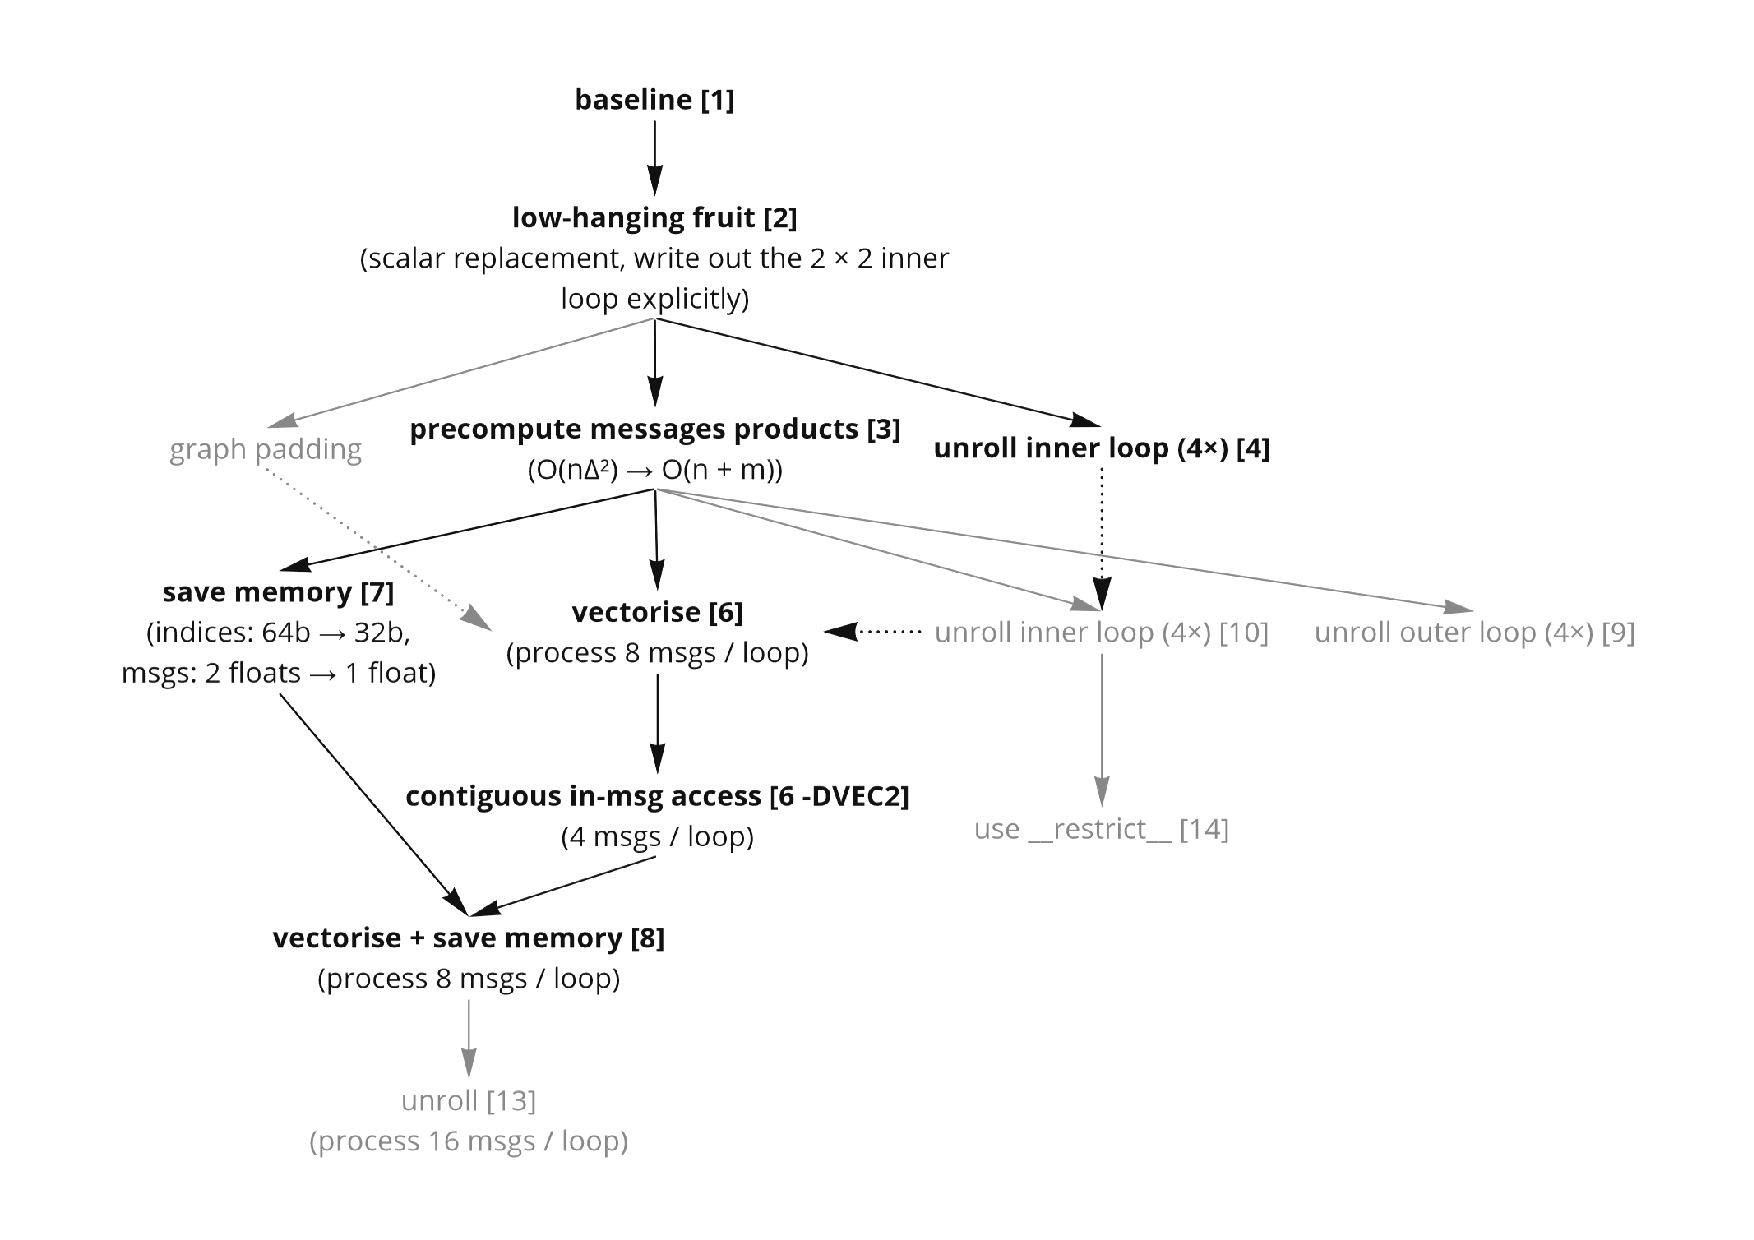
\includegraphics[trim=40 40 40 40, clip, width=0.72\textwidth]{img/OptimizationDiagram.pdf}
	\caption{Diagram of optimisation steps \label{OptDiagram}}
\end{figure*}

This section presents all optimisation steps seen in \cref{OptDiagram}.


\mypar{Baseline \opt{1}}
This project has two baselines. The first makes use of the C++ library libDAI, which implements belief propagation on a factor graph.
The second baseline, and basis for all optimisation, was implemented from scratch and strictly follows the belief propagation algorithm presented in \cref{sec:background}. It was implemented in a way that tries to maximize sequential array access and uses a CSR (compressed sparse row) inspired format for storing incoming messages.

Namely, we store a list $\arroff$ of vertex offsets. The incoming messages $m_{ji}$ of
vertex $i$ are stored in array $\arrin$ contiguously at indices $\arroff[i],
\ldots, \arroff[i + 1] - 1$. We additionally maintain an array $\arrout$ of
indices into $\arrin$, such that if $\arrin[k]$ represents message $m_{ij}$,
then $\arrin[\arrout[k]]$ represents message $m_{ji}$. This way, calculating the product of
incoming messages can be done contiguously, and random access is only needed
when sending a message to a neighbour.

\mypar{Low-hanging fruit \opt{2}}
The first optimisations applied on top of the baseline implementation were scalar replacement and writing out explicitly the inner two by two loops starting on line~\ref{line:for-xc} of \cref{algo:propagate}. This optimisation was then used as basis for all following steps.

Using scalar replacement for values that are accessed through pointers should allow the compiler to use more optimisations since the possibility of aliasing is excluded, and can possibly save memory accesses when a pointer is dereferenced once instead of multiple times.
Writing out the inner two by two loop saves on control flow instructions in addition to saving computation as well as enabling the compiler more predictability.

\mypar{Precompute message products \opt{3}} In the next step, we switched to
the asymptotically faster algorithm introduced in \cref{subsec:faster}. This
improved the time complexity from $\O(m\cdot \avgdeg)$ to $O(m + n)$, while
decreasing the flop count to $C(G) = 26m + 9n$\sr{This is not consistent with what you find in the end of sectio 2.3}. On the other hand, it
introduced additional division operations which have worse latency and
throughput.

\mypar{Graph padding}
In anticipation of unrolling and SIMD, optional graph padding was added to optimisation \opt{3}. The idea behind it was to add $\O(n)$ dummy edges to the graph that would not have any influence on the result, but would make the number of neighbours of a node divisible by 4 or 8 respectively.
As a consequence, vectorised code could use aligned instead of unaligned loads. Besides that, no small sequential leftover loop would be needed when the $j$-loop from \cref{algo:propagate} is unrolled and vectorised.
To see for every unrolling and vectorisation step whether the additional nodes or the leftover loop are the bigger overhead, the graph padding could be activated using a compiler flag (by default deactivated).
The graph padding was included in all successive optimisation steps.

\mypar{Unroll inner loop \opt{4 \& 10}}
Unrolling the inner loop, the $j$-loop in \cref{algo:propagate}, was done once on basis of optimisation \opt{2} and once on basis of optimisation \opt{3}. In both implementations, the loop was unrolled by a factor of~4. This allowed for more scalar replacement. Since the for-loop iterations are independent, computing all of them at once allows for more instruction level parallelism (ILP).
The difference in the two unrolling implementations is that thanks to optimisation \opt{3}, the second version unrolls a loop with much fewer computations, which means that ILP can be expected to have less impact. \sr{Henry, would you say we need a plot here too?} \st{since we are tight on space anyway, I could also leave out the last sentence}
\HT{If we would plot \opt{4}, it must be on one of those existing figures but I don't see it fitting anywhere} \st{Removed the sentence calling for a comparison between thees two}


\mypar{Unroll outer loop \opt{9}}
In a different implementation, based on optimisation \opt{3}, we examined what happens if the outer loop is unrolled. Specially, the $i$-loop from \cref{algo:propagate} was unrolled by a factor of 4. Since with optimisation \opt{3} the computation of messages product was pushed to the outer loop, it was of interest to see if unrolling this loop would allow for increased ILP. Or if, with 4 inner loops run during one unrolled iteration of the outer loop, the loss of locality would result in decreased performance.

\mypar{Vectorise \opt{6}}
\rh{do we need ``as seen''?} \st{no, removed it}SIMD was introduced on top of \opt{3}. First, Intel AVX2 intrinsics for vector instructions were introduced that very closely followed the instruction sequence of scalar computation. This way, 8 messages were processed together per loop iteration.

In a second step, the vector instructions were optimised with shuffling in-messages after loading them into vector registers to have more sequential access. Additionally, the number of messages handled during one iteration was reduced to 4. \st{maybe I should go into more detail here}\sr{pherhaps it would be interesting}
 
Even though, looking at the assembly compiled from optimisation \opt{3}, it is visible that the compiler already introduced some vector instructions, writing them explicitly should allow for a greater use of SIMD. 
\HTinline{I think we should mention that even though only 4 msgs are processed, sequential in-msg access gives us a slight performance increase. (maybe in section 4 with plot?)}



\begin{comment}
For this course, explain all the optimisations you performed. This mean, you first very briefly
explain the baseline implementation, then go through locality and other optimisations, and finally SSE (every project will be slightly different of course). Show or mention relevant analysis or assumptions. A few examples: 1) Profiling may lead you to optimise one part first; 2) bandwidth plus data transfer analysis may show that it is memory bound; 3) it may be too hard to implement the algorithm in full generality: make assumptions and state them (e.g., we assume $n$ is divisible by 4; or, we consider only one type of input image); 4) explain how certain data accesses have poor locality. Generally, any type of analysis adds value to your work.

As important as the final results is to show that you took a structured, organized approach to the optimisation and that you explain why you did what you did.
\end{comment}

\mypar{Save memory \opt{7}}
Since it was reasonable to assume that memory accesses would also be a limiting factor in performance, the number of unnecessarily loaded bytes were reduced. This was done in two places.

The LIKE and DISLIKE states have to add up to 1 according to the algorithm definition. This means, instead of storing two states, we could store only 1 and compute the other with a simple subtraction, saving a memory access.

In a second step, the type of indices was changed from \verb@size_t@ to \verb@uint32_t@. This is sufficient for any input that needs less than 48 GB of memory. 
\rh{these line breaks (\\) are kind of weird, are they needed?} \st{I had some strange issues with paragraph spacing, but seems to work without them now}

This compaction allowed for more values being read when loading 1 cache block, making memory access more efficient.


\mypar{Combine vectorisation and saving memory\opt{8}}
In the next step, optimisation \opt{6} and \opt{7} were combined. This optimisation was expected to work well together, since it combines greater computational efficiency with greater memory efficiency. Additionally, the number of messages processed per iteration was increased to 8, to account for the increased data efficiency.


\mypar{Unroll \opt{13}}
On basis of optimisation \opt{8} another unrolling was tested. Now, the number of messages processed per iteration was increased from 8 to 16. The idea was to see if we could make more use of optimisation \opt{7} to increase ILP \rh{suggestion: ``if we/one could make (even) more use of optimisation \opt{7} and increase ILP even more'', the passive voice is cumbersome here} \st{thanks}  or if this would lead to a loss of locality and slow down computation.


\mypar{Use \_\_restrict\_\_ \opt{14}}
In a next step, based on optimisation \opt{10}, the \verb@__restrict__@ keyword was used to ensure that the compiler did not make any assumptions about memory aliasing and therefore hindering some optimisations.

%Now comes the ``beef'' of the paper, where you explain what you
%did. Again, organize it in paragraphs with titles. As in every section
%you start with a very brief overview of the section.
%
%For this course, explain all the optimizations you performed. This mean, you first very briefly
%explain the baseline implementation, then go through locality and other optimizations, and finally SSE (every project will be slightly different of course). Show or mention relevant analysis or assumptions. A few examples: 1) Profiling may lead you to optimize one part first; 2) bandwidth plus data transfer analysis may show that it is memory bound; 3) it may be too hard to implement the algorithm in full generality: make assumptions and state them (e.g., we assume $n$ is divisible by 4; or, we consider only one type of input image); 4) explain how certain data accesses have poor locality. Generally, any type of analysis adds value to your work.
%
%As important as the final results is to show that you took a structured, organized approach to the optimization and that you explain why you did what you did.
%
%Mention and cite any external resources including library or other code.
%
%Good visuals or even brief code snippets to illustrate what you did are good. Pasting large amounts of code to fill the space is not good.


\section{Evaluation}\label{sec:exp}
\rhinline{Maybe Experimental evaluation?}\sr{If you like that much better, just change it}

\oldlinewidth=\linewidth
\begin{figure*}[!t] % Don't know how to get rid of the !, but it works somehow
\begin{minipage}[t]{\oldlinewidth}\centering
	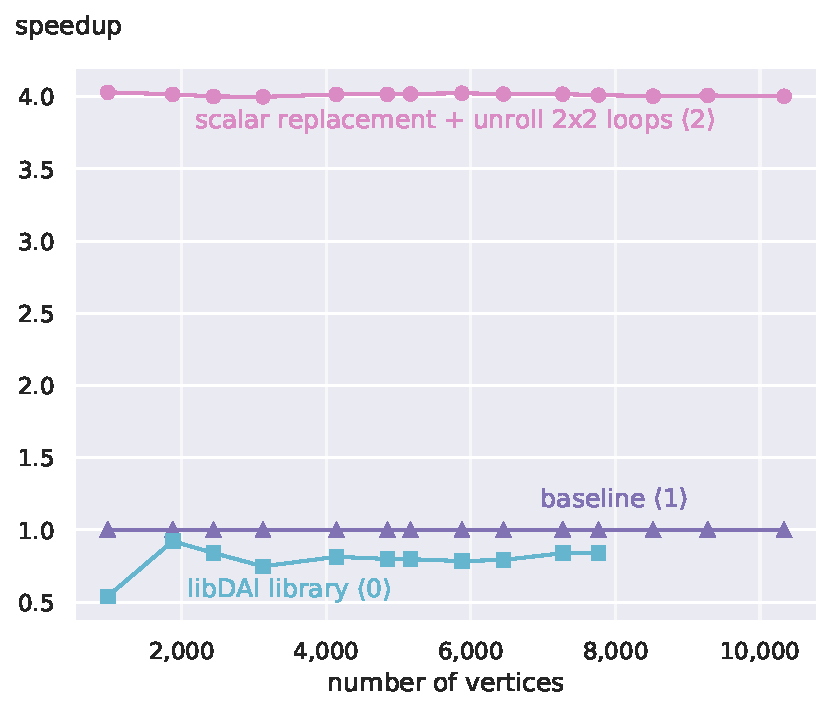
\includegraphics[width=\linewidth]{img/speedup[0][1][2]_small.pdf}
	\caption{Relative speedup of optimisation step \opt{2} and the libDAI library \opt{0} over the baseline \opt{1} on the small dataset. \label{libSpeedupSmall}}
\end{minipage}%
\hspace{7.2mm}
\begin{minipage}[t]{\oldlinewidth}\centering
	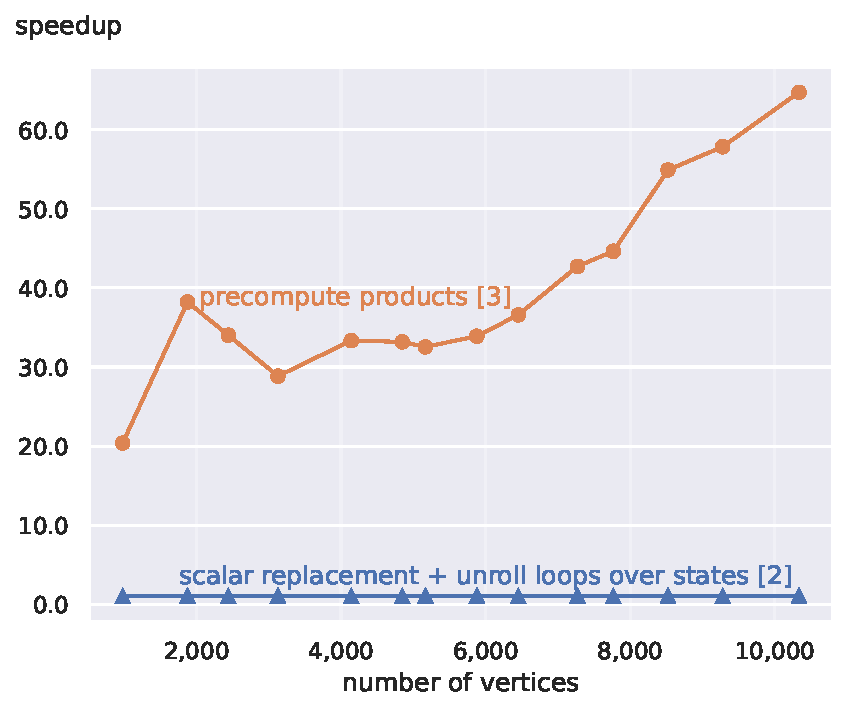
\includegraphics[width=\linewidth]{img/speedup[2][3]_small.pdf}
	\caption{Relative speedup of optimisation step \opt{3} over optimisation \opt{2} on the small dataset. \label{precomputeSpeedupSmall}}
\end{minipage}%
\end{figure*}


This section starts by describing the experimental setup in the first part.
In the second part, we show the results of our experiments evaluating the optimisations steps described in the previous section. 

\subsection{Experimental setup}\label{sec:setup} This \namecref{sec:setup} provides details about the experimental setup by describing the platform and compiler used, the test inputs and how measurements were performed. 

\mypar{Platform} All the experiments were conducted on an Intel(R) Core(TM) i5-7200U @2.50GHz machine which is described in \cref{platform}.
\begin{table}
	\begin{tabularx}{\linewidth}{ 
			@{} % <-- to get rid of the space on the left
			>{\raggedright\arraybackslash}l
			>{\raggedright\arraybackslash}X 
			@{} % <-- the same for the right space
		}
		\textbf{Processor}	&	Intel(R) Core(TM) i5-7200U														\\
		\textbf{Code name}	&	Kaby Lake \cite{intelSpec}														\\
		\textbf{Cores}		&	2 \cite{intelSpec}																\\
		\textbf{Threads}	&	4 \cite{intelSpec}																\\
		\textbf{Frequency} 	&	2.50GHz (Turbo Boost disabled)													\\
		\textbf{L1 cache} 	& 	2 x 32 KB 8-way set associative instruction cache \cite{optimisationManual}		\\
							&	2 x 32 KB 8-way set associative data cache \cite{optimisationManual}	 		\\
		\textbf{L2 cache}	&	2 x 256 KB 4-way set associative cache \cite{optimisationManual}				\\
		\textbf{L3 cache}	&	3 MB 12-way set associative shared cache \cite{cpuWorldSpec, intelSpec}			\\
		\textbf{RAM} 		&	2 × 8 GB DDR4 2133 MT/s 														\\
	\end{tabularx}
	\caption{Experimental platform \label{platform}}
\end{table} 
The processor specification states a maximum overall memory bandwidth of 34.1 GB/s for two channels \cite{intelSpec}.
Halving this number gives 17.05 GB/s per channel in theory.
For comparison, \cref{streamBenchmarkResults} shows best memory throughput rates actually measured on this platform for a single core using John D. McCalpin's STREAM memory benchmark \cite{streamBenchmark1,streamBenchmark2}.
\begin{table}
	\begin{tabularx}{\linewidth-5mm}{ 
		    @{}
			>{\raggedright\arraybackslash}X
			>{\raggedright\arraybackslash}X
			@{}
		}
		\textbf{Function}	&	\textbf{Best Rate [MB/s]}   \\ \hline
		Copy 				&	14,273.6					\\
		Scale				&	13,646.1					\\
		Add 				&	16,250.3					\\
		Triad				& 	16,047.6 					\\
	\end{tabularx}
	\caption{Memory throughput of experimental platform for a single core measured using John D. McCalpin's STREAM memory benchmark \cite{streamBenchmark1,streamBenchmark2}.\label{streamBenchmarkResults}}
\end{table}
Taking the average over all functions in \cref{streamBenchmarkResults} gives 15'054.4 MB/s which is around 15 GB/s.
Dividing this 15 GB/s by 2.5 GHz, results thus in an average memory bandwidth $\beta=6$ bytes/cycle. 
Furthermore, the bandwidths for L1, L2 and L3 caches are 81, 29 and 18 bytes/cycle according to \cite{optimisationManual}.

\mypar{Compiler flags} The program was compiled using GCC 12.1.0 with \verb@g++ -Ofast -march=native@.

% Small (n, 2m)
% 981 2076
% 1879 5560
% 2442 8064
% 3128 14548
% 4142 23068
% 4847 30780
% 5167 36818
% 5879 49794
% 6452 64728
% 7272 84366
% 7766 99904
% 8522 116802
% 9278 139318
% 10334 166976

% Big (n, 2m)
% 45729 4018282
% 71223 8236252
% 92295 12399882
% 111227 16542254
% 135339 20754570
% 152638 24861856
% 169867 28990694
% 187172 33030750
% 204131 37153852
% 221003 41289484
% 221588 41436056
\mypar{Input data} Test inputs were based on the MovieLens dataset \cite{movieLens}.
Various sizes were generated by taking the ratings of users with identifier smaller than some number for different numbers
and then normalising / desparsifying the user and movie identifiers separately, mapping them to $\{1, \ldots, \#\text{users}\}$ and $\{1, \ldots, \#\text{movies}\}$ respectively.\rh{added this here to clarify, but not sure if clear enough}\HT{I think it is sufficient}
This section's plots display the results of either a small or a big dataset composed from inputs generated this way.
The small dataset represents graphs with $\approx$1--10k vertices and $\approx$1--80k edges based on the MovieLens Latest Small dataset \cite{movieLensSmall}. %and consists of inputs 981, 1'879, 2'442, 3'128, 4'142, 4'847, 5'167, 5'879, 6'452, 7'272, 7'766, 8'522, 9'278, 10'334 
%considering the first 10, 20, 30, 60, 90, 120, 150, 210, 270, 330, 390, 450, 540 and 610 users  
The big dataset represents graphs of $\approx$40k--200k vertices with $\approx$2--20 million edges based on the MovieLens 25M dataset \cite{movieLensBig}. %and considers the first 16,200, 32,400, \dots, 162,000 users (taking steps of 16,200)
\HT{Maybe just saying ``981 to 10,334 vertices and 1,038 to 83,488 edges`` is enough and leave out the user counting (ditto for big data). The Input data subsection seems too much for my taste. What do you think?}\sr{Yes, I feel similarly}

\mypar{Measurement} For measuring the number of cycles, the \verb@RDTSC@ instruction has been used.
In addition, the number of flops has been calculated directly in the measurement code.
\rh{This is sloppy, but I think we should mention it. If you can improve on it, please do.}\sr{I think this fits into the methods section.} As mentioned in \cref{subsec:topn}\sr{Is this what you wanted RH?}, we solely optimised and measured the belief propagation procedure of \cref{algo:propagate}.
The number of iterations was set to 10 with the exception of optimisations \opt{1, 2} measured on the big dataset.
In those cases, only a single iteration was run due to the runtime growing prohibitively large otherwise.

\subsection{Experimental results}  The subsequent paragraphs demonstrate the incremental performance and runtime improvements achieved by successively applying the optimisations described in \cref{sec:yourmethod}.
Additionally, interesting failed attempts are discussed.  
Finally, a roofline plot with the final optimisation step and the relative end-to-end speedup over the baseline \opt{1} are shown.

\begin{figure*}[!t]
\begin{minipage}[t]{\oldlinewidth}\centering
	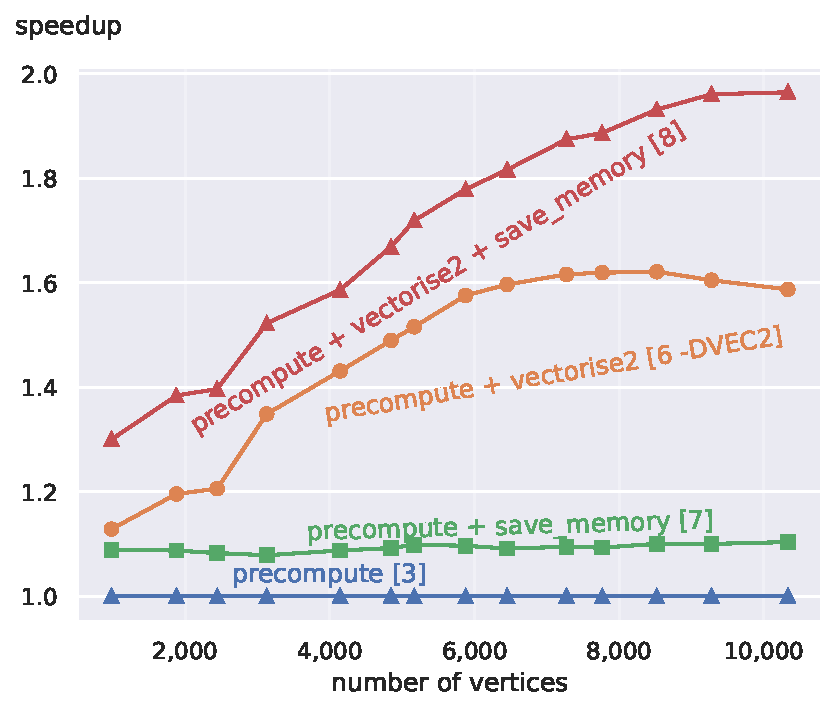
\includegraphics[width=\linewidth]{img/speedup[3][6][7][8]_small.pdf}
	\caption{Relative speedup of vectorisation and saving memory optimisation steps over optimisation \opt{3} on the small dataset. \label{cpctVectSpeedupSmall}}
\end{minipage}%
\hspace{7.2mm}
\begin{minipage}[t]{\oldlinewidth}\centering
	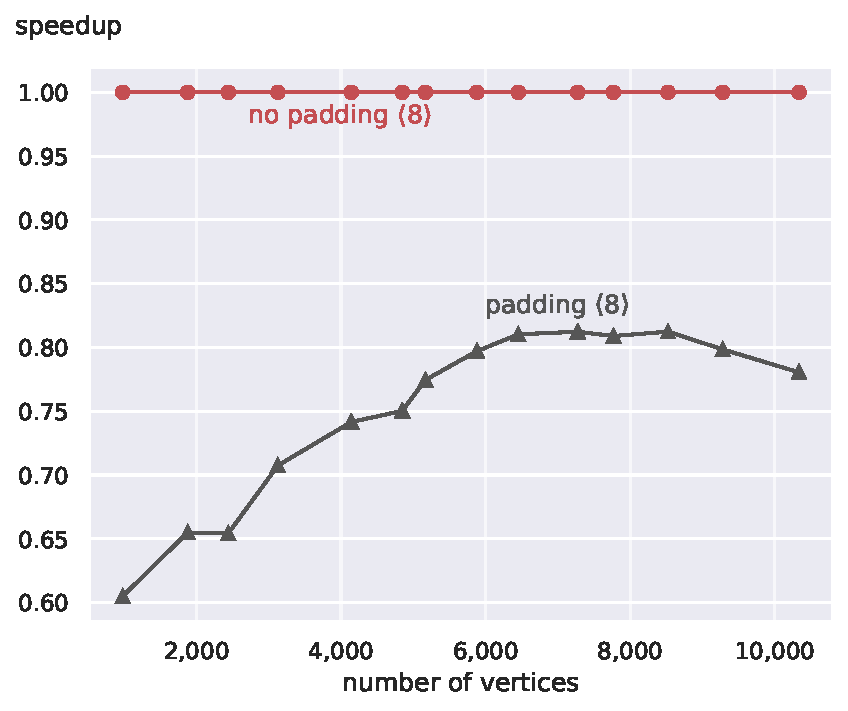
\includegraphics[width=\linewidth]{img/speedup[8]padding_small.pdf}
	\caption{Relative speedup of using graph adding on top of optimisation step \opt{8} on the small dataset. \label{speedupGraphPaddingSmall}}
\end{minipage}%

\begin{minipage}[t]{\oldlinewidth}\centering
	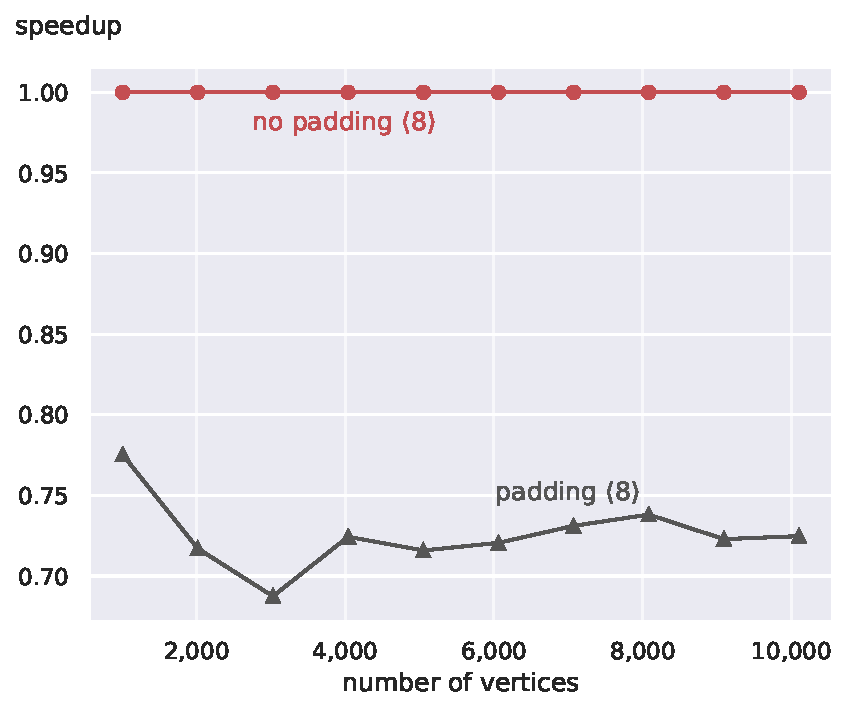
\includegraphics[width=\linewidth]{img/speedup[8]padding_bipartite.pdf}
	\caption{Relative speedup of using graph adding on top of optimisation step \opt{8} on complete bipartite graphs. \label{speedupGraphPaddingBipartite}}
\end{minipage}%
\hspace{7.2mm}
\begin{minipage}[t]{\oldlinewidth}\centering
	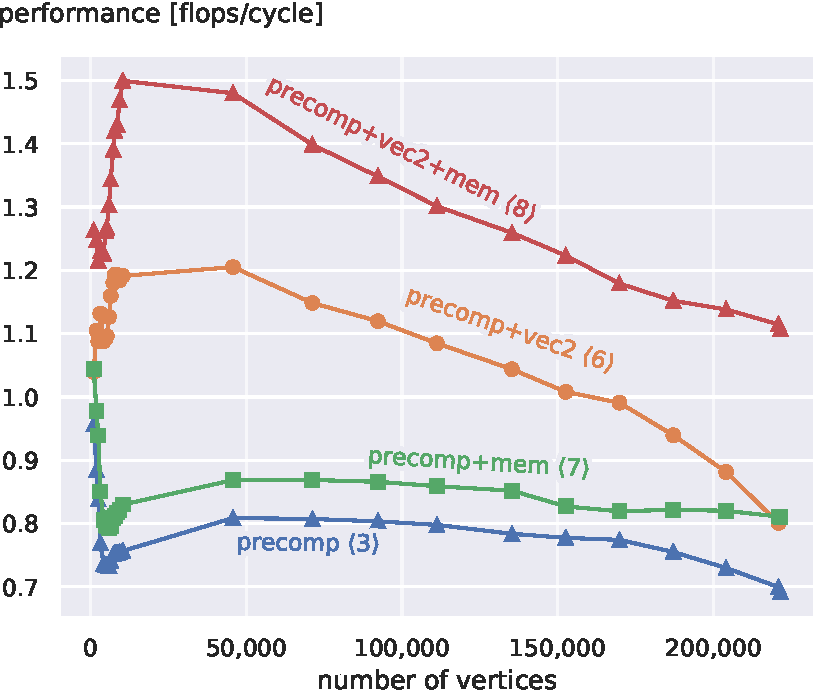
\includegraphics[width=\linewidth]{img/performance[3][6][7][8]_both.pdf}
	\caption{Performance of optimisations \opt{3}, \opt{6}, \opt{7} and \opt{8} on the small and big dataset combined. \label{cpctVectPerformanceBoth}}
\end{minipage}%
\end{figure*}
\rh{Fig 4: saving memory $\to$ memory reduction?}\sr{Where do you see 'saving memory'? I think I just used 'mem'.}

\mypar{Base implementation / optimisation} Since there are two base implementations, one implemented from scratch and the other using the libDAI library, it is interesting to see which one is faster.
For this purpose, the relative speedup in runtime of the different base implementations over the from scratch implementation on the small dataset is displayed in \cref{libSpeedupSmall}.
We see that libDAI library \opt{0} uses the most cycles compared to the others.
Already implementing the algorithm from scratch provided slight runtime benefits (baseline \opt{1} in \cref{libSpeedupSmall}).
Presumably, this came from the benefits of not using a library: less bound checks and function calls, and inlining of functions.
Another reason is that baseline \opt{1} was implemented in a way to maximize sequential array access and used a CSR inspired format for storing all the incoming messages.
Applying optimisation \opt{2} to the baseline \opt{1} gives a 4$\times$ speedup.
One reason for this is that the product calculation at line~\ref{line:calc-prod-slow} of the algorithm can be reused by the outer loop iterating over states. 
Another important reason is scalar replacement, which eliminates many pointer dereferences.

\mypar{Reducing computation} Optimisation step \opt{3} reduced floating point operations,
but also introduced divisions, which is bad because division has worse latency and throughput than addition/multiplication on the target machine.
\cref{precomputeSpeedupSmall} shows that on the small dataset, optimisation step \opt{3} achieves a relative speedup of at least $20\times$ over optimisation \opt{2}.
This is because the average degree is large enough that the cost of the introduced division is offset by improved time complexity.

\begin{figure*}[!t]
\begin{minipage}[t]{\oldlinewidth}\centering
	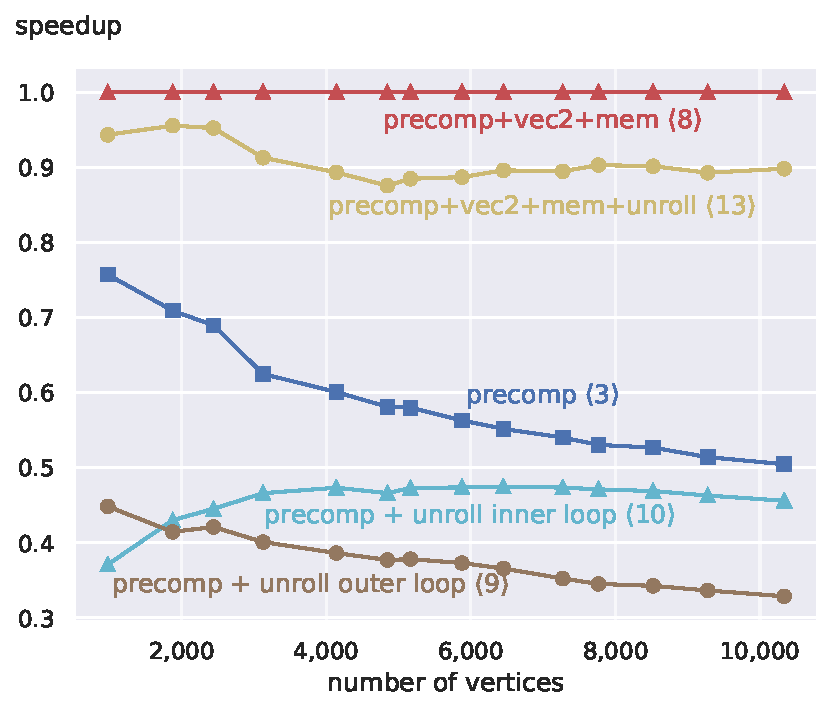
\includegraphics[width=\linewidth]{img/speedup[3][8][9][10][13]_small.pdf}
	\caption{Relative speedup of further unrolling added on top of optimisation step \opt{3} by optimisations \opt{9,10} respectively optimisation \opt{13} on top of optimisation step \opt{8} on the small dataset. \label{speedupUnsuccessful}}
\end{minipage}%
\hspace{7.2mm}
\begin{minipage}[t]{\oldlinewidth}\centering
	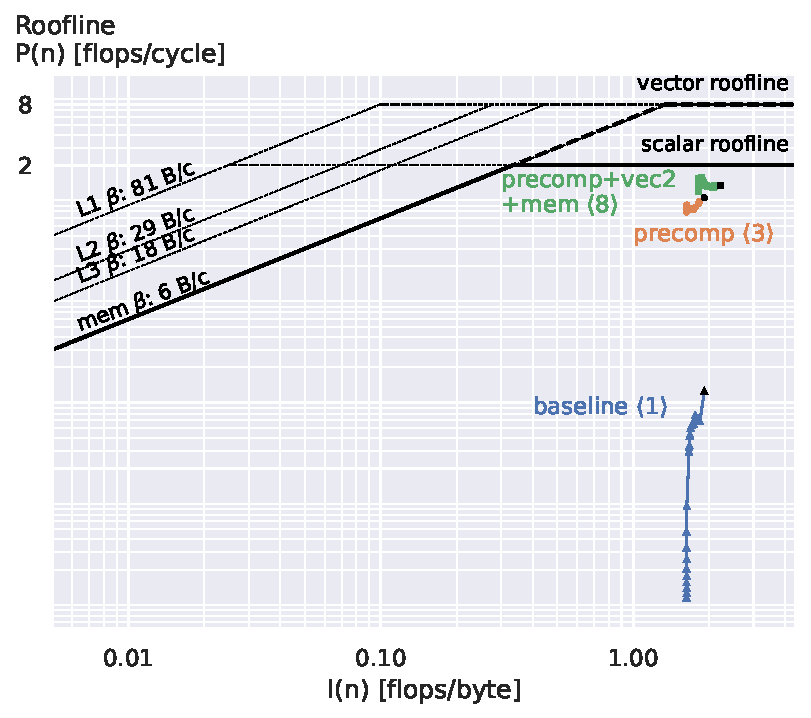
\includegraphics[width=\linewidth]{img/roofline[1][3][8]_both.pdf}
	\caption{Roofline plot of optimisation steps \opt{8}, \opt{3} and the baseline \opt{1} on the small and big dataset combined.
	Black dots represent the smallest input n.
	The rooflines are with respect to scalar / vectorized peak processor performance (2 resp. 8 flops/cycle) and the bandwidths of L1,L2,L3 and memory mentioned in \cref{sec:setup} \emph{Platform}.
	We assumed each random access has to load a cache line from main memory. \label{rooflineEndToEnd}}
\end{minipage}%
\end{figure*}
\begin{figure}[!bt]\centering
	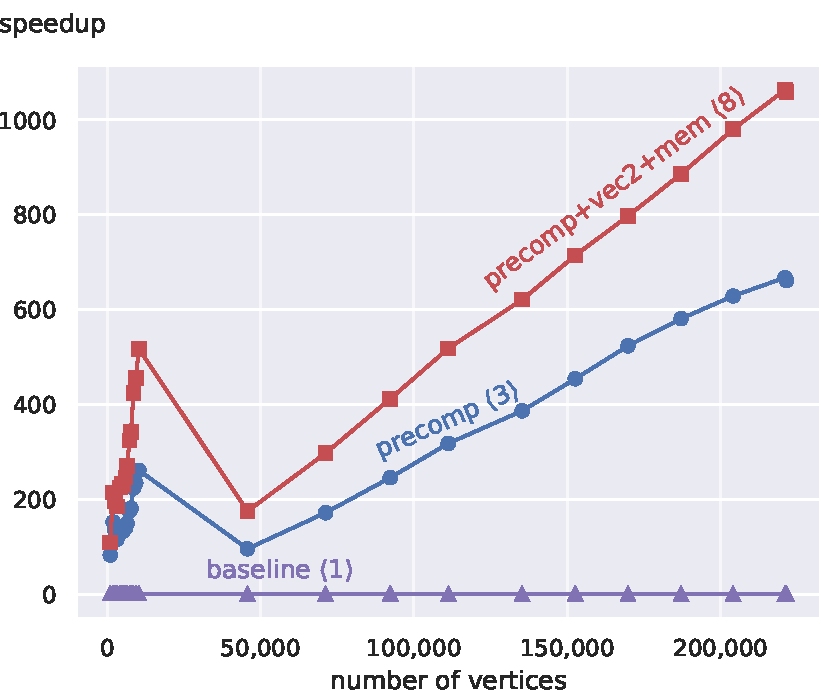
\includegraphics[width=\linewidth]{img/speedup[1][3][8]_both.pdf}
	\caption{Relative end-to-end speedup over baseline \opt{1} on the small and big dataset combined} \label{speedupEndToEnd}
\end{figure}\sr{Does mentioning the assumption fit here, Richard?}

\mypar{Saving memory and vectorisation} 
For further improvement on top of optimisation \opt{3}, optimisation \opt{7} tried to reduce the memory footprint and optimisation \opt{6} added vectorisation.
We see in \cref{cpctVectSpeedupSmall} a relative speedup of around 1.1$\times$ for reducing the memory footprint while vectorisation yields a relative speedup of 1.1--1.6$\times$ with respect to optimisation \opt{3} on the small dataset.
The relative speedup of the combined version of both optimisations (optimisation \opt{8} in \cref{cpctVectSpeedupSmall}) is 1.3--2$\times$ which is greater than each of them separately.

\mypar{Graph padding} To examine the effect of SIMD alignment we tried to pad the graph so that the list of neighbours / incoming messages for each vertex starts on an address divisible by SIMD size.
In \cref{speedupGraphPaddingSmall}, we see graph padding is slower compared to optimisation step \opt{8}.
The latency and throughput on the platform do not differ between unaligned and aligned vectorised load.
Therefore, using aligned loads did not benefit the relative speedup.
Apart from that, graph padding increases the memory footprint and introduces excess computation.
If padding is needed for most of the vertices, the memory overhead becomes significant.\rh{if I understand it this sentence correctly, that's not necessarily true, the padding is done so that the size will be exactly a multiple of SIMD size, so no leftover loop is needed (in the last iteration, we just maybe deal with some dummy edges which is fine, the SIMD algo doesn't mind).}\sr{Sorry, this was the moment when I forgot I was writing a paragraph about graph padding and only thought of vectorsation. Removed the whole sentence.}
Since our test input data is sparse, we wanted test whether the negative effects on speedup are decreased on graphs of large average degrees.\rh{This sounds weird, for what reason? AFAIK the reason is only described later (we want to (dis)prove that bigger avg degree might work) and that's why it's weird. But I can't think of how to reformulate}\sr{What do you think about the paragraph now?}
To this end, \cref{speedupGraphPaddingBipartite} displays the relative speedup over optimisation step \opt{8} measured on complete bipartite graphs.
\Cref{speedupGraphPaddingBipartite} disproves the idea that padding could result in greater relative speedup on graphs of large average degree: 
The gap in relative speedup on bipartite graphs is not significantly decreased compared to \cref{speedupGraphPaddingSmall}.
\srinline{It turns out for the small dataset we used, considering all users, the average degree of a vertex is on average 165.3 and after edge thresholding 89.72 on average.}\rh{how did you arrive at those numbers? My calculations say something different}\sr{Maybe this sentence has become superflous now.}

\mypar{Other unsuccessful optimisations} Optimisations \opt{9,10} tried to increase ILP of optimisation step \opt{3} by unrolling the outer respectively the inner loop four times.
Optimisation \opt{13} tried to achieve the same thing by unrolling the inner loop sixteen times but based on \opt{8}.
\Cref{speedupUnsuccessful} shows that these optimisation steps could not increase the speedup relative to the optimisation steps they emerged from.
Presumably, unrolling the outer loop resulted in worse locality whereas for the inner loop, the leftover loops have more iterations and possibly register spilling occurred.\sr{*}\rhinline{is that the case though? for unroll-i I think bad locality definitely plays a bigger role. For unroll-j, tbh, I don't know. the division may be a factor, but I don't think that's the full story. Maybe we spill out of registers? or, in case of vectorisation, spend more time in leftover loop because it's larger on average?}
%Therefore, unrolling by factors of more than 8\sr{ (?)*} does not improve the relative speedup.
Optimisation step \opt{14} using the restrict keyword is not shown in this plot as it almost coincides with the line representing optimisation step \opt{10} which it was based on.
This suggests the code already runs as fast as if no pointer aliasing was assumed without using the keyword.

\mypar{Performance \& Big inputs} The optimisations displayed in \cref{cpctVectSpeedupSmall} constitute the final successful steps taken.
Therefore, it is interesting to finally see the actual performance achieved.
In addition, we only discussed what happens on the small dataset so far.
To get a more complete view, \cref{cpctVectPerformanceBoth} shows the performances of these optimisations on the small and big dataset combined.
With the big dataset, the working set that doesn't fit into cache anymore.
We see that for the bigger inputs the combined version is still the best but the memory saving has a much bigger impact on speedup.
The vectorised versions drop faster than the non-vectorised versions as their advantages in efficient computation get drowned out by slow memory accesses.
All the optimisations displayed surpass the performances of the base implementations (mentioned in \cref{libSpeedupSmall}), whose performances were all below 0.05 flops/cycle (below 0.005 flops/cycle on the big dataset).
For all versions, starting from the datapoint close to 50,000 vertices, the data structures didn't fit into L3 cache anymore.

\mypar{Roofline}
Optimisation step \opt{8} is the final one.
In order to see whether it is memory or compute bound and how close it is to the optimal performance, consider \cref{rooflineEndToEnd}.
It is obvious from \cref{rooflineEndToEnd} that all versions reside in the compute-bound region.
The last optimisation step achieves around 16.13\% of the vectorised peak performance and 64.5\% of the scalar peak performance on average on the platform.  

\mypar{End-to-end speedup} To see the runtime gain achieved overall, \cref{speedupEndToEnd} displays the relative speedup over the baseline \opt{1} on the small and big dataset merged.
On the small dataset, the overall relative speedup lies between 100 to 500$\times$ for optimisation step \opt{8}.
The big dataset appears after the first peak in \cref{speedupEndToEnd}, after which the relative speedup scales with input size.\sr{*}
The peak is there because the different datasets have different average degree when starting from small inputs.
Since optimisation step \opt{3} was the last to have performed a major algorithmic optimisation, it is displayed for reference as well in \cref{speedupEndToEnd}.

%Here you evaluate your work using experiments. You start again with a
%very short summary of the section. The typical structure follows.

%\mypar{Experimental setup} Specify the platform (processor, frequency, cache sizes)
%as well as the compiler, version, and flags used. I strongly recommend that you play with optimisation flags and consider also icc for additional potential speedup.

%Then explain what input you used and what range of sizes. The idea is to give enough information so the experiments are reproducible by somebody else on his or her code.

%\mypar{Results}
%Next divide the experiments into classes, one paragraph for each. In the simplest case you have one plot that has the size on the x-axis and the performance on the y-axis. The plot will contain several lines, one for each relevant code version. Discuss the plot and extract the overall performance gain from baseline to best code. Also state the percentage of peak performance for the best code. Note that the peak may change depending on the situation. For example, if you only do additions it would be 12 Gflop/s
%on one core with 3 Ghz and SSE and single precision floating point.

%Do not put two performance lines into the same plot if the operations count changed significantly (that's apples and oranges). In that case first perform the optimisations that reduce op count and report the runtime gain in a plot. Then continue to optimise the best version and show performance plots.

%{\bf You should}
%\begin{itemize}
%\item Follow to a reasonable extent the guide to benchmarking presented in class, in particular
%\item very readable, attractive plots (do 1 column, not 2 column plots
%for this class), proper readable font size. An example is below (of course you can have a different style),
%\item every plot answers a question, which you pose and extract the
%answer from the plot in its discussion
%\end{itemize}
%Every plot should be referenced and discussed (what does it show, which statements do
%you extract).

\section{Conclusion}

In this paper, we focused on optimising the sequential performance belief propagation for top-n recommendation in C.
Top-n recommendation plays important role in online shopping, video and streaming platforms.\rh{drop}\sr{I just dropped the 'nowadays' did you mean the whole sentence?} 
We achieved a 100$\times$\rh{1000?}\sr{no, this is not true for all of our inputs} speedup on an Intel(R) Core(TM) i5-7200U @2.50GHz machine and on average 16.13\% vectorised peak performance on dataset which does not fit entirely into cache.
The speedup scales with input size such that for our greatest input containing more than 200,000 vertices, it exceeds 1000$\times$.\sr{should we mention this, since we scaled the measurements for the baseline?}\rh{I think the scaling up is relatively legit. After rerunning the experiments, 1 and 10 iterations behaved the same. So this is a ``real'' achievement IMO.}
For bigger inputs advantages in efficient computation get gradually drowned out by slow memory access.
Reducing the memory footprint of data structures at the expense of more computation had shown to have positive impact on speedup in this case.
Despite the divisions being introduced by our algorithmic optimisation and the fact that they limit the amount of instruction level parallelism beneficial significantly, this tradeoff suited the type of our input data very well and achieved the greatest relative speedup out of all optimisation steps.\sr{*}\rh{Maybe focus less on details and more on the takeaway message? hmm, but what is it? probably sth along the lines of ``the best optimisation was to improve the algorithm/time complexity'', but idk how to phrase it nicely}
\sr{*}\rh{would omit in this form because it's kind of negative :) but if we can formulate in some insightful manner, idk, ``we suspect we could improve it if we did this / if we had a machine with better this''}
%Here you need to briefly summarize what you did and why this is
%important. {\em Do not take the abstract} and put it in the past
%tense. Remember, now the reader has (hopefully) read the paper, so it
%is a very different situation from the abstract. Try to highlight
%important results and say the things you really want to get across
%(e.g., the results show that we are within 2$\times$ of the optimal performance ...
%Even though we only considered the DFT, our optimisation
%techniques should be also applicable ....) You can also formulate next
%steps if you want. Be brief.


\section{Contributions}% of Team Members (Mandatory)

%In this mandatory section (which is not included in the 8 pages limit) each team member should very briefly (telegram style is welcome) explain what she/he did for the project. I imagine this section to be between one column and one page (absolute maximum).

%Include only 
%\begin{itemize}
%	\item What relates to optimising your chosen algorithm / application. This means writing actual code for optimisation or for analysis.
%	\item What you did before the submission of the presentation.
%\end{itemize}
%Do not include
%\begin{itemize}
%	\item Work on infrastructure and testing.
%	\item Work done after the presentation took place.
%\end{itemize}

%Example and structure follows.

\mypar{Henry} Implemented flop counting in code. Tried out unrolling outer loop over nodes further. Tried out unrolling inner loop over neighbours of a node further. Extended flop counting with e.g. byte counting. Measured graph padding on bipartite graph. Implemented roofline plot. Helped with preparing plots for the presentation, mainly the roofline.

\mypar{Sarah} Implemented flop counting in code of both algorithms together with Henry. Improved library flop counting. Performed unrolling optimisation of inner loop over neighbours of a node. Mostly prepared the slides on optimisations for the presentation.

\mypar{Richard} Did the base implementation from scratch in C.
% in a favourable way maximizing sequential array access and using a CSR inspired format for storing incoming messages. % It's too long
Performed unrolling optimisation of innermost $2\times2$ loops over states and scalar replacement. Implemented precomputation of product optimisation. Tried graph padding optimisation. Helped Henry implementing/improving the roofline plot. Mostly prepared the slides on cost measure, experimental setup. Performed measurements and prepared plots.

\mypar{Stephanie} Did the base implementation using the libDAI library. Vectorised loop iterating over neighbours of a node. Implemented saving memory optimisation as discussed. Tried out restrict keyword and compiler flags. Mostly prepared slides on algorithm and cost measure for the presentation.

\srinline{Just wrote down what came into my mind so far. Most likely the description is incomplete and some points are wrong. Fix it.}

\section{Global TODOs}

\rhinline{just a list of TODOs we should tackle before submitting, feel free to add/disagree}

\subsection{Plots}

\rhinline{the supervisor seemed like he wanted to see more of big dataset plots? It kind of makes sense given that the small plots don't even overflow to RAM.}

\subsection{Typography/language/details to check before submitting}

\todo[inline]{save the PDF as \texttt{41\_report.pdf}}
\todo[inline]{disable slugs}
\todo[inline]{BrE vs AmE (RH has a script somewhere)}
\todo[inline]{spellcheck}
\todo[inline]{check there are no more TODOs hiding}
\todo[inline]{generally check the title, abstract, section titles, that we have no more template text somewhere}
\todo[inline]{minor details: use cref where appropriate, $\O$ instead of $O$, \texttt{hello} instead of `hello`, \opt{x} instead of [], 5$\times$ instead of 5x}
\todo[inline]{citations: don't use just plain URL when possible (usually everyone has a ``how to cite us'' section}
\todo[inline]{pdfgrep ``??'' (unresolved references)}

% References should be produced using the bibtex program from suitable
% BiBTeX files (here: bibl_conf). The IEEEbib.bst bibliography
% style file from IEEE produces unsorted bibliography list.
% -------------------------------------------------------------------------
%\bibliographystyle{IEEEbib}
\bibliographystyle{IEEEtranN}
\bibliography{bibliography}

\end{document}
